% Created 2023-01-18 Wed 23:30
% Intended LaTeX compiler: pdflatex
\documentclass[a4paper,12pt,twoside,twocolumn]{article}
\usepackage[utf8]{inputenc}
\usepackage{graphicx}
\usepackage{amsmath}
\usepackage{amssymb}
\usepackage{hyperref}
\usepackage[margin=2cm]{geometry}
\usepackage[sorting=none]{biblatex}

\addbibresource{references/references.bib}
\usepackage{listings}
\usepackage{xcolor}
\definecolor{commentgreen}{RGB}{2,112,10}
\definecolor{eminence}{RGB}{108,48,130}
\definecolor{weborange}{RGB}{255,165,0}
\definecolor{frenchplum}{RGB}{129,20,83}
\definecolor{soft_red}{RGB}{179,20,20}
\lstset{language=Python, frame=tb, tabsize=4, showstringspaces=false, numbers=left, commentstyle=\color{commentgreen}, keywordstyle=\color{eminence}, stringstyle=\color{red}, basicstyle=\small\ttfamily, emph={if,elif,else,def,class}, emphstyle={\color{soft_red}}, escapechar=\&, classoffset=1, otherkeywords={>,<,.,;,-,!,=,~}, morekeywords={>,<,.,;,-,!,=,~}, keywordstyle=\color{weborange}, classoffset=0}
\date{}
\title{Applied machine learning system ELEC0134 22/23 report SN: 17062315}
\hypersetup{pdfborder=0 0 0}

\begin{document}

\setlength\parindent{0pt}
\maketitle

\section{Abstract}
\label{sec:orgf9cd8ab}

Artificial Intelligence is evolving faster than ever. One domain in particular, computer vision has benefited from a vast amount of data annotated in the past decades and many recent breakthroughs on the software level.\\

It is now time to develop our own tool built on these discoveries. Its purpose is to tackle challenges in the face recognition area by analysing multiple features of the human face such as its shape, eyes and mouth which are essential to identify individuals and their emotions.\\

To reach this objective, we rely on annotated data in the form of pictures of celebrities and cartoonish characters.\\

The information from these datasets are then extracted and cleaned before being trained by various algorithms such as Support Vector Machine, Random Forests, K-nearest neighbour or bagging. The first two represent good alternatives to more complex algorithms such as neural networks and deep learning which imitate the way human learn in order to make the algorithm able to differentiate individuals.\\

Results are obtained by testing more than 20 variations of models against a subset of the dataset left aside for this specific purpose.\\

Upon completion of this project, it should be possible to take these proofs of concepts and embed them in more complex systems such as smart cameras and robots which are the most common kind of devices which may benefit from an improved perception.\\

\section{Introduction}
\label{sec:org673447e}

Last century, science fiction authors such as Isaac Asimov predicted the rise of intelligent devices \autocite{asimov_akinyemi_2000} \autocite{ai_eco_impact} and now, the dawn of artificial intelligence is upon us. After, the Tay bot \autocite{tay}, it is now the turn of ChatGPT to earn an immense popularity among tech enthusiasts with its ability to provide detailed answers to any question \autocite{chatgpt-detect} \autocite{chatpgt-teach}. And to add to this triumph, Microsoft has shown interest in acquiring OpenAI, the creator of ChatGPT and many other AIs \autocite{microsoft_buy_openai}.\\

But while everyone has their eyes on this new chatbot, a more discrete, albeit, just as interesting revolution, has been ongoing for a few decades already in the computer vision domain.\\

The first visible step toward it was the introduction of captcha \autocite{captcha_original} in 1997. These challenge-response tests quickly became annotation tools channelling the efforts of humans to train artificial intelligences \autocite{captcha_recognition}.\\

Applications are numerous, ranging from biometric tests to disease detection \autocite{cv_cancer} and even robotics with the latest self driving cars \autocite{cv_robotics}.\\

In this report, we shall pay close attention to a specific use case: face recognition. After mentioning the latests relevant breakthroughs, we shall see how we can design softwares able to recognise the gender, emotions, face shape and eye colour of various celebrities and cartoonish characters.\\

\section{Literature survey}
\label{sec:orga3b40b8}
Face recognition has been a major topic recently with new algorithms and tools appearing in quick successions as early as last century with, for instance, the creation of Support Vector Machines in 1992, algorithms shining for their adaptability and generalisation ability  \autocite{face_recognition_svm} \autocite{app_svm} or OpenCV created in 2000 and which is a library still widely used in many languages such as C++ and Python \autocite{opencv_face_detect}.\\

Many algorithms were used over the years such as Support Vector Machine and K-nearest neighbour \autocite{recognition_algos}. They all come with their advantages and trade-offs. Convolutional neural networks especially tend to be studied with great attention because of their ability to imitate the human mind which has been AI's goal since its inception \autocite{face_detect_cnn} \autocite{thermal_cnn}.\\

Since various algorithms exist, the main objective nowadays shifted from pure scientific research to engineered solutions to deal with edge cases where computer vision still struggles \autocite{face_reading}.\\

Firstly, faces become harder to analyse with low resolution images and and dim lighting which make data extraction less precise \autocite{gender_classify_facehop}.\\

Moreover noise is more important with data obtained from pictures of people belonging to specific demographic subgroups such as old males, people with darker skin types \autocite{face_detect_disparity} or children which tend to appear as androgynous since gender only becomes more apparent past puberty \autocite{gender_classify_children}.\\

These problems can generally be also explained by biased datasets which contain unbalanced representation of said demographic subgroups \autocite{face_detect_bias}.\\

It is therefore essential to handle data preprocessing with as much care as the analysis itself as we will see in the next sections.\\

\section{Models Description}
\label{sec:org495de86}

CNN are considered as the most efficient model overall out of the one we studied. Which is why we should not rely on them in this report as it is more interesting to not know how a model fares. We will therefore study other popular models including SVMs, Bagging, KNN (K nearest neighbours) and Random Forests and determine which is the best among them for each task.\\

\subsection{Support Vector Machines}
\label{sec:orge78b144}

\begin{center}
\begin{figure}[htbp]
\centering
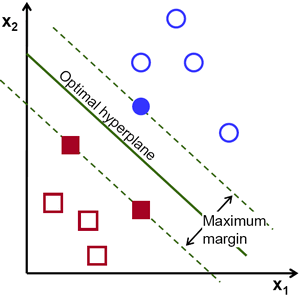
\includegraphics[width=.9\linewidth]{./images/svm.png}
\caption{SVM algorithm}
\end{figure}
\end{center}

The first model, SVM, is very robust for both classification and regression in supervised learning tasks. Their purpose is to find a hyperplane that best divides a dataset into two classes.\\

For instance, with a linear SVM, we seek w and b such that \(\rho = \frac{2}{\|w\|}\) is maximised and for all \((x_i, y_i), i = 1...n: y_i(w^T x_i + b) \geq 1\).\\

This leads to a quadratic problem where we want \(\phi(w) = w^Tw\) minimised for the aforementioned values of \(x\) and \(y\).\\

The solution is a dual problem with a Lagrange multiplier \(\alpha_i\) summarised as \(f(x) = \sum \alpha_i y_i x_i^Tx + b\) with every non-zero \(a_i\) indicating the presence of a support vector in the form of \(x_i\).\\

One of the most important benefits of SVM is their ability work both on linear and multiclass problems with a kernel which can be fine tuned to deal with a specific problem. Most of the time, a standard Polynomial or RBF kernel for multi class problems.\\

\subsection{Random Forest}
\label{sec:orga340817}

\begin{center}
\begin{figure}[htbp]
\centering
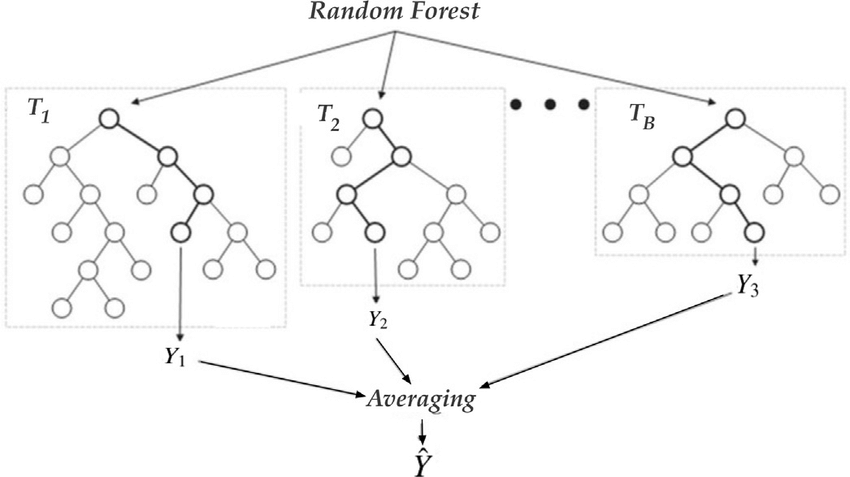
\includegraphics[width=.9\linewidth]{./images/forest.png}
\caption{Random forest algorithm}
\end{figure}
\end{center}

Another model are decision trees which consist in putting if conditions in cascade to find a solution. It relies on the theory of entropy \(H(x) = - \sum_{x \in S_x} p_x(x) log p_x (x)\) which is a measure of disorder obtained when many parameters shape a solution.\\

But random trees tend to converge slowly which is why fancier alternatives such as bagging or random forests are used. In the case of Random Forests, a number of decision trees is created based on bootstrapped training samples.\\

Each time a split in a tree is considered, a random sample of \(q\) attributes is chosen as split candidates from the full set of \(p\) attributes as its optimal value is data dependant. The branches are averaged at the end.\\

\subsection{Bagging}
\label{sec:org572cc01}

When decision trees fail because of overfitting, we can instead rely on ensemble methods such as bagging which can help by decreasing variance of the base model without influencing bias at the cost of a loss of simple structures in comparison to the original model.\\

In the case of bagging, we pick a base learning model and apply it over many samples. Classification is done by majority vote and also uses a training set consisting of many examples for various models used to get an aggregate overall model.\\

\subsection{KNN}
\label{sec:org76563aa}

\begin{center}
\begin{figure}[htbp]
\centering
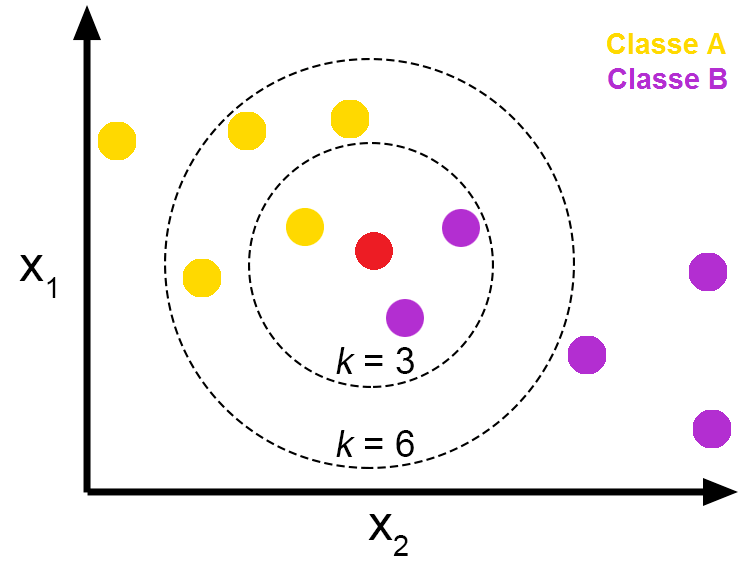
\includegraphics[width=.9\linewidth]{./images/knn.png}
\caption{KNN algorithm}
\end{figure}
\end{center}

Finally, K-nearest neighbour algorithms rely on the entire training set. It relies on a metric \(\rho\) that returns a distance between two points such as the Euclidean distance \(\sqrt{\sum_{k=1}^d_{}^{} (x_k - x_k')^2}\) . It is relatively simple and will always converge at the expense of performance since it needs to solve a very expensive distance problem.\\

\section{Implementation}
\label{sec:orga8e233c}

Because of the decision taken to compare 4 famous models, the code displays a decoupled nature so that every task can call any model. This leads to a very simple main file similar to the simplified version shown below:\\

\lstset{language=Python,label= ,caption= ,captionpos=b,numbers=none}
\begin{lstlisting}
task = task_class.task
various_data = task.main_properties

X, y = extract_features_labels(...)
models, results = multi_train_test(...)
plot_data(...)
\end{lstlisting}

Every task class hold information essential to find the dataset associated to it. With them, it is possible to start extracting features by taking each image from the appropriate dataset directory, detecting its landmarks by greying the image and using 68 data points from a predictor.\\

Also, if a binary model is used with values equal to -1 or 1, it is essential to normalise them to 0 or 1 in prevision of the training which relies on positive data to avoid bias.\\

\lstset{language=Python,label= ,caption= ,captionpos=b,numbers=none}
\begin{lstlisting}
def extract_features_labels(...):
    ...
    for imgage_index ...:
	img = image.img_to_array(...)

    features, _ = run_dlib_shape(img)

    if req_label in ["gender", "smile"]: 
	lbl = (np.array(all_labels) + 1)/2
\end{lstlisting}

The next part of the code is the split\_train\_test() function which is used to save cpu cycles. Since my laptop is quite slow, testing models with 10000 images in a short amount of time is not reasonable.\\

Because of that, the training data is cut in two parts for training and testing. This also removes the need to rely on a second dataset for testing. By default, a split of 75\% or 80\% of training and the rest for testing has yielded good results.\\

\lstset{language=Python,label= ,caption= ,captionpos=b,numbers=none}
\begin{lstlisting}
def split_train_test(X, y, prop_train):
    ...
    return tr_X, tr_Y, te_X, te_Y ...
\end{lstlisting}

With the split obtained, training can start. This is the most important part of the code. It is a function which can make predictions with any classifier provided.\\

\lstset{language=Python,label= ,caption= ,captionpos=b,numbers=none}
\begin{lstlisting}
def general_classifier(img,lb,clf)    
    classifier.fit(training data)
    pred = classifier.predict(test)
    return accuracy_score(...)
\end{lstlisting}

It really shines when combined with a function called multi\_train\_test() which calls a random forest, KNN and bagging 9 times with parameters ranging from 1 to 9 and the 4 most common SVM kernels (linear, polynomial, rbf and sigmoid).\\

This way we obtain 23 models which are then compared so that only the best of each category remain to be plotted which allows us to determine easily how well they perform for each task.\\

\section{Experimental Results and Analysis}
\label{sec:orgad48b21}
\subsection{Task A1}
\label{sec:org07506da}

\begin{center}
\begin{figure}[htbp]
\centering
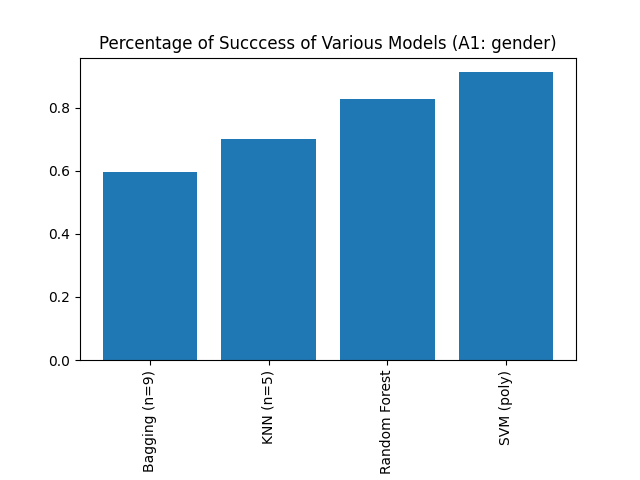
\includegraphics[width=.9\linewidth]{./images/A1: gender.png}
\caption{Task A1: gender (5000 images)}
\end{figure}
\end{center}

\begin{center}
\begin{tabular}{lr}
Model & Accuracy\\
\hline
Bagging (n=9) & 0.5975\\
KNN (n=5) & 0.7\\
Random Forest & 0.8275\\
SVM (poly) & 0.914\\
\end{tabular}
\end{center}

For task 1, most models performed reasonably well as the worst one obtained barely less than 60\% of accuracy. SVM obtained the best results which is withing expectation as it is the main alternative to CNN in term of efficiency. The only unusual point worth noting is that the poly kernel ended up being the most efficient which is surprising as the linear kernel is tailored for binary classifiers.\\

\subsection{Task A2}
\label{sec:org2a9c81f}

\begin{center}
\begin{figure}[htbp]
\centering
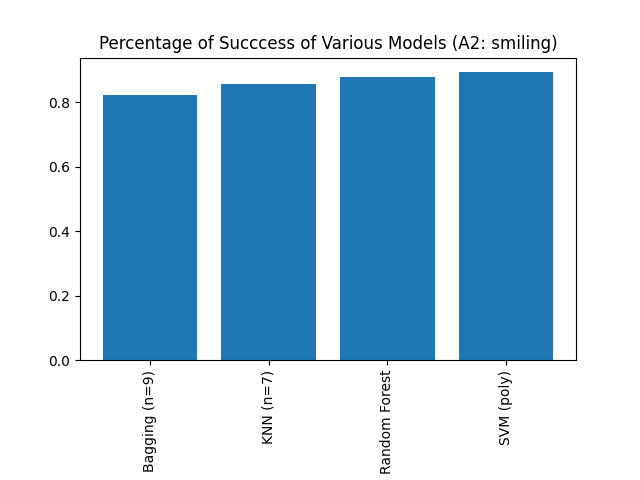
\includegraphics[width=.9\linewidth]{./images/A2: smiling.png}
\caption{Task A2: emotion (5000 images)}
\end{figure}
\end{center}

\begin{center}
\begin{tabular}{lr}
Model & Accuracy\\
\hline
Bagging (n=9) & 0.824\\
KNN (n=7) & 0.856\\
Random Forest & 0.878\\
SVM (poly) & 0.894\\
\end{tabular}
\end{center}

This task is the one with the best overall results probably related to the fact that smiles tend to be easier to recognise vector wise than gender as they correspond to a curve which is easy to represent mathematically. Because of this, there is not much difference between the predictions from all models which are all in the 80\% of success range.\\

\pagebreak\\
\subsection{Task B1}
\label{sec:org886e2d7}

\begin{center}
\begin{figure}[htbp]
\centering
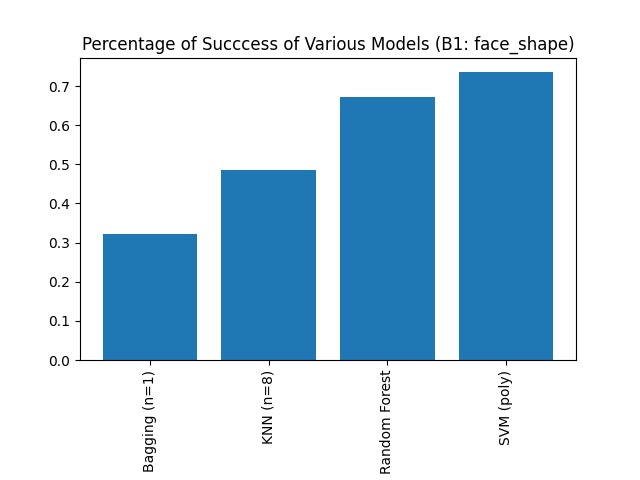
\includegraphics[width=.9\linewidth]{./images/B1: face_shape.png}
\caption{Task B1: Shape (5000 images)}
\end{figure}
\end{center}

\begin{center}
\begin{tabular}{lr}
Model & Accuracy\\
\hline
Bagging (n=1) & 0.321\\
KNN (n=8) & 0.487\\
Random Forest & 0.672\\
SVM (poly) & 0.736\\
\end{tabular}
\end{center}

With the halved training dataset due to my computer's limitations and the addition of more possible values, most models performed noticeably less well. As per usual, the SVM with polynomial kernel got some good result and the random forest came as a close second as it is technically a more refined version of trees / bagging and does not suffer from the KNN limitation which overall needs even more data to compensate the difficulty to obtain distances with the possible values multiplied by a factor 2.5 in comparison to task A.\\

\subsection{Task B2}
\label{sec:orgdf070f1}

\pagebreak\\


\begin{center}
\begin{figure}[htbp]
\centering
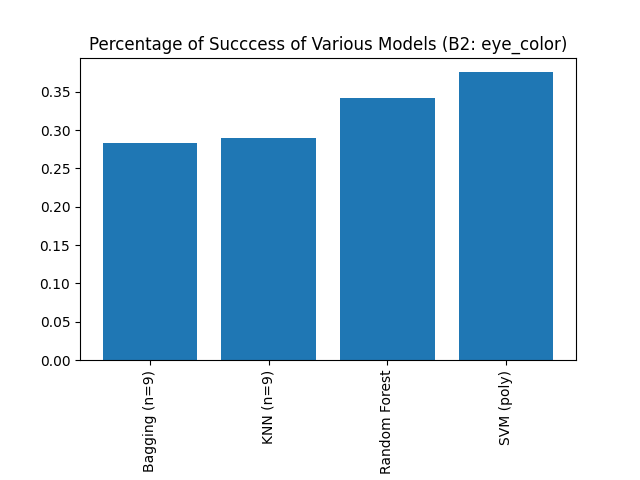
\includegraphics[width=.9\linewidth]{./images/B2: eye_color.png}
\caption{Task B2: Eyes color (5000 images)}
\end{figure}
\end{center}

\begin{center}
\begin{tabular}{lr}
Model & Accuracy\\
\hline
Bagging (n=9) & 0.284\\
KNN (n=9) & 0.289\\
Random Forest & 0.342\\
SVM (poly) & 0.376\\
\end{tabular}
\end{center}

Finally, this task was the most arduous for all models. Identifying eye colour on a grey scaled image is relatively hard even for a human and this is where getting more powerful models such as a CNN really makes a difference. One important point to add is that many characters from the cartoon dataset wear sunglasses which absolutely biases the result by adding unusable data.\\

\subsection{Improvements}
\label{sec:orgd5515c8}

From these results, we can infer that Random Forests and SVM perform better than the two other models which are either less refined in the case of bagging or simply too dependant on wide datasets with few possible values for KNN.\\

In order to get better results, more preprocessing would have been necessary for the cartoon dataset which ended up being harder to analyse for all models.\\

Regarding Support Vector Machines, the algorithm performed relatively well for every task as it constantly emerged on top. For further tests, it would be better to keep it and try to conceive a custom kernel for task B2 on which it did not perform well.\\

Additionally, fine tuning with weight alteration and modification of the cost function always remains an option for SVM as long as it does not lead to overfitting by making the result mostly correlated to a subset of the training data\\

And if it does not suffice, switching to neural networks or deep learning remains a valid option.\\

\section{Conclusion}
\label{sec:org1f1c890}

Hence, if really paid off to try multiple algorithms as out of all the algorithms tested, Support Vector Machines emerged as the most reliable in term of performance and flexibility with their polynomial or custom kernel.\\

Random forests come as a close second while the other models do not perform well enough to represent an alternative to a neural network.\\

We may try next time to mix different strategies such as K-means clustering which is extremely slow and therefore inefficient but which has the advantage of converging with absolute certitude.\\

Moreover, a more promising alternative would be to try more Deep Learning strategies which imitate the way human learn and work particularly well in tandem with neural networks.\\

Thankfully, the results gathered from the present research should pave the way to better softwares combining them with other strategies such as reinforcement learning in robots and self driving car which could therefore both recognise humans and learn how to drive around them.\\

\pagebreak\\

\vfill \pagebreak \printbibliography \vfill\null\\
\pagebreak \vfill\null \pagebreak\\

\section{Appendix (github link and code output)}
\label{sec:orgc6f95d3}

This is the output obtained when running the four tasks with 5000 images.\\

\subsection{A1}
\label{sec:org2688140}

\begin{verbatim}
: Working on task A1 with label gender from dataset celeba
: Proceeding to get 5000 images including 0.75% for training
: 
: 100% 5000/5000 [01:57<00:00, 42.63it/s]
: Bagging (n=9) 0.5975
: KNN (n=5) 0.7
: Random Forest 0.8275
: SVM (poly) 0.9141666666666667
\end{verbatim}

\subsection{A2}
\label{sec:orgda19819}

\begin{verbatim}
: Working on task A2 with label smiling from dataset celeba
: Proceeding to get 5000 images including 0.75% for training
: 
: 100% 5000/5000 [01:57<00:00, 42.66it/s]
: Bagging (n=9) 0.8241666666666667
: KNN (n=7) 0.8558333333333333
: Random Forest 0.8783333333333333
: SVM (poly) 0.8941666666666667
\end{verbatim}

\subsection{B1}
\label{sec:orgcca7483}

\begin{verbatim}
: Working on task B1 with label face_shape from dataset cartoon_set
: Proceeding to get 5000 images including 0.75% for training
: 
: 100% 5000/5000 [08:58<00:00,  9.29it/s]
: Bagging (n=1) 0.3209028459273798
: KNN (n=8) 0.4867517173699706
: Random Forest 0.6722276741903828
: SVM (poly) 0.7360157016683022
\end{verbatim}

\subsection{B2}
\label{sec:org14069be}

\begin{verbatim}
: Working on task B2 with label eye_color from dataset cartoon_set
: Proceeding to get 5000 images including 0.75% for training
: 
: 100% 5000/5000 [08:59<00:00,  9.27it/s]
: Bagging (n=9) 0.28361138370951916
: KNN (n=9) 0.28949950932286556
: Random Forest 0.34151128557409227
: SVM (poly) 0.3758586849852797
\end{verbatim}

\pagebreak \vfill\null \pagebreak\\

\subsection{Github Link}
\label{sec:orgd46ca3e}

Github: \url{https://github.com/Ubunteous/applied-ml-final-version}\\
\end{document}